\documentclass[onecolumn, draftclsnofoot,10pt, compsoc]{IEEEtran}
\usepackage{graphicx}
\usepackage[section]{placeins}
\usepackage{url}
\usepackage{setspace}
 
%For indentItem command
\usepackage{enumitem}
\usepackage{changepage}

%For \textrightarrow
\usepackage{textcomp}
\usepackage{tgpagella}
 
%For Gantt Chart
\usepackage{xspace}
\usepackage{pgfgantt}
\usepackage{subcaption}
 
\usepackage{alltt}                                           
\usepackage{float}
\usepackage{color}
\usepackage{url}

\usepackage{geometry}
\geometry{textheight=9.5in, textwidth=7in}
\setlength\parindent{0pt}

\usepackage{xspace}
\usepackage{pgfgantt}
\usepackage{subcaption}

% 1. Fill in these details
\def \CapstoneTeamName{\textbf{Insert Team Name Here} }
\def \CapstoneTeamNumber{8}
\def \GroupMemberOne{James Stallkamp}
\def \GroupMemberTwo{Jeremy Fischer}
\def \GroupMemberThree{Austin Row}
\def \CapstoneProjectName{Kora}
\def \CapstoneSponsorCompany{Autodesk}
\def \CapstoneSponsorPerson{Patti Vrobel}
\def \botname{Kora\xspace}
\def \speechToText{WIT.ai\xspace}

\newenvironment{indentItem}[1][1cm]{\begin{adjustwidth}{#1}{}}{\end{adjustwidth}}

% 2. Uncomment the appropriate line below so that the document type works
\def \DocType{		%Problem Statement
				%Requirements Document
				%Technology Review
				Design Document
				%Progress Report
				}

\newcommand{\designConcernDef}[3]{
    \subsection{#1}
        \begin{tabular}[t]{r p{6in}}
            Stakeholder(s): & #2 \\
            Concern: & #3 \\
        \end{tabular}
}
\newcommand{\designConcernRef}[2][]{
    #2 #1
}
\newcommand{\designElementDef}[4]{
    \subsubsection{#1}
    \begin{tabular}[t]{r p{6in}}
        Type: & #2 \\
        Purpose: & #3 \\
        Author: & #4 \\
    \end{tabular}
}
\newcommand{\designElementRef}[2]{
    \subsubsection{#1}
    \begin{tabular}[t]{r p{6in}}
        See #2 & \\ %#2 should be element identifier (section where it's defined or ID that can be used to find it)
    \end{tabular}
}
\newcommand{\NameSigPair}[1]{\par
\makebox[2.75in][r]{#1} \hfil 	\makebox[3.25in]{\makebox[2.25in]{\hrulefill} \hfill		\makebox[.75in]{\hrulefill}}
\par\vspace{-12pt} \textit{\tiny\noindent
\makebox[2.75in]{} \hfil		\makebox[3.25in]{\makebox[2.25in][r]{Signature} \hfill	\makebox[.75in][r]{Date}}}}
% 3. If the document is not to be signed, uncomment the RENEWcommand below
\renewcommand{\NameSigPair}[1]{#1}

%%%%%%%%%%%%%%%%%%%%%%%%%%%%%%%%%%%%%%%
\begin{document}
\begin{titlepage}
    \pagenumbering{gobble}
    \begin{singlespace}
    	\includegraphics[height=4cm]{coe_v_spot1}
        %\hfill 
        % 4. If you have a logo, use this includegraphics command to put it on the coversheet.
        \par\vspace{.2in}
        \centering
        \scshape{
            \huge CS Capstone \DocType \par
            {\large\today}\par
            \vspace{.5in}
            \textbf{\Huge\CapstoneProjectName}\par
            \vfill
            {\large Prepared for}\par
            \Huge \CapstoneSponsorCompany\par
            \vspace{5pt}
            {\Large\NameSigPair{\CapstoneSponsorPerson}\par}
            {\large Prepared by }\par
            Group\CapstoneTeamNumber\par
            % 5. comment out the line below this one if you do not wish to name your team
            %\CapstoneTeamName\par 
            \vspace{5pt}
            {\Large
                \NameSigPair{\GroupMemberOne}\par
                \NameSigPair{\GroupMemberTwo}\par
                \NameSigPair{\GroupMemberThree}\par
            }
            \vspace{20pt}
        }
        \begin{abstract}
			This Document describes the design views and components of \botname.
			The document begins by introducing definitions, purpose, scope, context, and a summary for the overall project.
			After the introduction the document lists stakeholders and their concerns.
			The rest of the document is divided into sections which each provide a different design viewpoint.
			These different viewpoints show how the specified design addresses the concerned laid out previously. 
        \end{abstract}     
    \end{singlespace}
\end{titlepage}
\newpage
\pagenumbering{arabic}
\tableofcontents
% 7. uncomment this (if applicable). Consider adding a page break.
%\listoffigures
%\listoftables
\clearpage

% 8. now you write!


\section{Frontspiece}
	\subsection{Date of Issue and Status}
		This document was issued November 30, 2017 and is the first draft of the design document.
	
	\subsection{Issuing Organization}
		This document has been issued by Oregon State University and Autodesk via the senior design capstone class.
	
	\subsection{Authorship}
		Jeremy Fischer, Austin Row, and James Stallkamp are the authors of this document and the developers of Kora.
		
	\subsection{Change History}
		\begin{table}[H]
			\centering
			\caption{Change History}
			\label{my-label}
			\begin{tabular}{|l|l|}
				\hline
				\textbf{Date}     & \textbf{Change Description}   \\ \hline
				November 30, 2017 & {First design document draft} \\ \hline
			\end{tabular}
		\end{table}

\section{Introduction}
	\subsection{Purpose}
		The purpose of this design document is to outline how Kora's workflows will be completed and connected.
		More generally, this document describes how the client's requirements will be met.
		Kora's developers will use this document as a roadmap during implementation.

	\subsection{Scope}
		This document focuses on the relationships between Kora's components and their individual processes, and how they work together to satisfy the project's requirements.
	
	
	\subsection{Summary}
		Kora will be a speech-based virtual assistant for Fusion that lets users perform any one of a subset of tasks within the product, such as saving a document or opening a menu, by verbally instructing it to perform the task.
		Workflows in Fusion that are not suited for handling by a voice interface will not be supported by Kora.
		As a stretch goal, Kora will be capable of questioning the user and using responses to predict and automatically assist with future user behavior.
		It will be a plugin that is bundled with Fusion and will be part of the product's standard download. 
		
		Kora will offer users a tool that decreases the time required to achieve their goals within Fusion by offering an interface that runs in parallel with and complements the keyboard and mouse.
		If the stretch goal is achieved, Kora will further increase productivity by learning to predict and automate specific workflows within the product.

\section{Glossary}
	\begin{table}[H]
		\centering
		\caption{Glossary}
		\label{my-label}
		\begin{tabular}{|l|l|}
			\hline
			\textbf{Term} & \textbf{Definition} \\ \hline
			Kora & The virtual assistant that is the focus of this project \\ \hline
			NLP & Natural Language Processing \\ \hline
			API & Application Programing Interface \\ \hline
			CAD & Computer Aided Design \\ \hline
			CAM & Computer Aided Manufacturing \\ \hline
			Fusion & An Autodesk Cloud-based 3D CAD/CAM tool/product \\ \hline
			Task & In the context of Fusion, a function or operation that can be performed in Fusion \\ \hline
			Plugin & Software that adds specific new functionality to another piece of software \\ \hline
			User & A person that interacts with Kora or Fusion depending on the context \\ \hline
			Workflow & A sequence of related tasks \\ \hline
		\end{tabular}
	\end{table}

\section{Design Stakeholders and Concerns}
    \designConcernDef{User-Application Interface}{Client, Developers}{What interfaces will exist for users to communicate to the application and for the application to communicate to users?}
    \designConcernDef{Internal Interfaces}{Developers}{What internal interfaces will exist in the software system?}
    \designConcernDef{Component Interactions}{Developers}{Which components of the software system will interact?}
    \designConcernDef{Component Interaction Responsibilities}{Developers}{What are the responsibilities of each component of the software system in the context of interactions?}
	\designConcernDef{Architecture}{Developers}{How is the system structured?}

%%%%%%%%%%%%%%%%%%%%%%%%%%%%%%%%%%%%%%%%%%%%%%%%%%%%%%%%%%%%%%%%%%%%%%%%%%%%%%%%%%%%%%%%%%%%%%%%%%%%%%%%%%% 
%                                           ***NOTES***
%
% Addressed Design Concerns:
%    1) Should specify by ID each of the concerns from the "Design Stakeholders and Concerns"
%       that are being addressed or discussed in that particular viewpoint.
%
% Design Elements: 
%    1) If element is not previously defined in other viewpoint, then offer definition. 
%       Otherwise reference definition in other viewpoint (e.g. "See 4.5.2")
%
% Design Rationale:
%    1) There won't be a single section for design rationale. As per the IEEE standards doc,
%       the design rationale should be justification for decisions made in the desing and
%       it doesn't need a dedicated section. Just make sure to include justification for 
%       why we chose to do something in a certain way (e.g. "Use of the Mediator design pattern
%       allows the application to...")
%%%%%%%%%%%%%%%%%%%%%%%%%%%%%%%%%%%%%%%%%%%%%%%%%%%%%%%%%%%%%%%%%%%%%%%%%%%%%%%%%%%%%%%%%%%%%%%%%%%%%%%%%%% 
\section{Design Viewpoint: Composition}
    \subsection{Addressed Design Concerns}
        \begin{itemize}
            \item \designConcernRef[]{Component Interaction Responsibilities}
        \end{itemize}

    \subsection{Design Elements} 
        \designElementDef{Manager Module}
                         {Module}
                         {Manages what state \botname is in and executes other modules.}
                         {James Stallkamp}
        \designElementDef{User Interface Module}
                         {Module}
                         {Provides input to \botname and expresses the state of \botname to the user.}
                         {James Stallkamp}
        \designElementDef{Speech-To-Intent Module}
                         {Module}
                         {Anaylzes speech input and produces an intent.json object.}
                         {James Stallkamp}
        \designElementDef{Logger Module}
                         {Module}
                         {Stores runtime and contextual information to be used for training \botname.}
                         {James Stallkamp}
        \designElementDef{Fusion API Module}
                         {Module}
                         {Translates intent into Fusion API commands and executes them.}
                         {James Stallkamp}
        \designElementDef{Voice Synthesizer Module}
                         {Module}
                         {Synthesizes an audio output from a given text input.}
                         {James Stallkamp}
        \designElementDef{Machine Learning Module}
                         {Module}
                         {Trains \botname to become a more powerful assistant.}
                         {James Stallkamp}
						 
    \subsection{Design View: Modules}
		\botname is composed of seven primary modules.
		\subsubsection{Manager Module}
			\begin{indentItem}
				The first module is the master module, this module is responsible for coordinating all other modules.
				The master module will contain definitions for functions needed to process data objects, other modules will inherit this from master.
			\end{indentItem}
		\subsubsection{User Interface}
			\begin{indentItem}
				The User interface is the module responsible for all interaction with the user.
				This module will collect input and communicate it to the master module as well output regular feedback to the user.
			\end{indentItem}
		\subsubsection{Speed-To-Intent Module}
			\begin{indentItem}
				The speech-to-intent module will take in audio input and output a json object containing information on the spoken input.
				This intent module will construct the json object and return it to master.
			\end{indentItem}
		\subsubsection{Logger Module}
			\begin{indentItem}
				The Logger module will initialize a persist able data object containing runtime information from \botname.
				Data logged will be used to help train and improve \botname.
			\end{indentItem}
		\subsubsection{}
			\begin{indentItem}
				The next module is the Fusion API, this module will handle executing Fusion commands.
				The Fusion module will translate information in the json data object to construct and execute a Fusion command.
			\end{indentItem}
		\subsubsection{Voice Synthesizer Module}
			\begin{indentItem}
				In order for \botname to output speed to the user it will need a voice synthesizer module.
				This module will receive text input and produce an audio output that can be played to the user.
			\end{indentItem}		
		\subsubsection{Machine Learning Module}
			\begin{indentItem}
				The last module is the machine learning module, this module is responsible for training \botname to recognize patters and improve functionality.
			\end{indentItem}
		
\section{Design Viewpoint: Information}
	\subsection{Addressed Design Concerns}
		\begin{itemize}
			\item
		\end{itemize}


	\subsection{Design Elements}
		\designElementDef{MongoDB}{Database}{Database to hold the log files}{Jeremy}
		\designElementDef{JSON object}{Storage structure}{The structure the information will be store in}{Jeremy}
		\designElementDef{HTTP calls}{Access mechanism}{How the data will be posted and accessed}{Jeremy}
	
	\subsection{Design View: Contents}
		The contents of the data will be:
		\begin{itemize}
			\item the intent generated by the Speech-to-Intent
			\item the context generated by the Speech-to-Intent such as quantities
			\item whether the user's request was successfully processed
			\item the date
			\item the time
			\item the user identification
		\end{itemize}
	
	\subsection{Design View: Access}
		The data will be posted and accessed via HTTP calls to the database.
	
	\subsection{Design View: Structure}
		The data will be stored in a MongoDB database.
		Each entry in the database will resemble the JSON object that is returned from the Speech-to-Intent module driver function.
		
		

\section{Design Viewpoint: Patterns}
    \subsection{Addressed Design Concerns}
        \begin{itemize}
            \item \designConcernRef[]{Architecture}
        \end{itemize}

    \subsection{Design Elements}
		\designElementDef{Mediator Framework}
						 {System Framework}
						 {\botname has a simple mediator that coordinates all interactions between all other components.}
						 {James Stallkamp}
		\designElementDef{Worker Class}
						 {Class}
						 {A inheritable class providing functionality to handle the json object}
						 {James Stallkamp}				 
    \subsection{Design View: }
		\botname is structured in a mediator format. 
		\botname will have a master module that coordinates interactions between itself and all other modules.
		This master module will provide basic functionality needed to process data objects, other modules will inherit this from master. 


\section{Design Viewpoint: Interfaces}
    \subsection{Addressed Design Concerns}
        \begin{itemize}
            \item \designConcernRef[User-Application Interface]{ID}
            \item \designConcernRef[Internal Interfaces]{ID}
        \end{itemize}

    \subsection{Design Elements}
        \designElementDef{Element-Name}{Element-Type}{Element-Purpose}{Element-Author}
        \designElementDef{UI Module Interface}{Internal Interface}{Defines rules governing interactions with the UI module.}{Austin Row}
        \designElementDef{Speech-to-Intent Module Interface}{Internal Interface}{Defines rules governing interactions with the Speech-to-Intent module.}{Austin Row}
        \designElementDef{Logging Module Interface}{Internal Interface}{Defines rules governing interactions with the Logging module.}{Austin Row}
        \designElementDef{Text-to-Speech Module Interface}{Internal Interface}{Defines rules governing interactions with the Text-to-Speech module.}{Austin Row}
        \designElementDef{Fusion Module Interface}{Internal Interface}{Defines rules governing interactions with the Fusion module.}{Austin Row}
        \designElementDef{Action Prediction Module Interface}{Internal Interface}{Defines rules governing interactions with the Action Prediction module.}{Austin Row}
        \designElementDef{Runtime Data Store Interface}{Internal Interface}{Defines rules governing interactions with the global Runtime Data Store.}{Austin Row}
    \subsection{Design View: Module Interfaces}
        The interfaces to each module are driven by a method, \textit{handle}, that takes a JSON variable, \textit{data}, as an argument.
        The required data transmitted in \textit{data} is specific to each module. 
        The following interface definitions describe the required contents of \textit{data} for each module.

        \subsubsection{UI Module Interface}
            \begin{tabular}[t]{r p{6in}}
                INPUT: & \\
                OUTPUT: & \\
            \end{tabular}

        \subsubsection{Speech-to-Intent Module Interface}
            \begin{tabular}[t]{r p{6in}}
                INPUT: &  \{ dataIDs: \}\\
                OUTPUT: & This module returns a \\
            \end{tabular}

\section{Design Viewpoint: Interactions}
    \subsection{Addressed Design Concerns}
        \begin{itemize}
            \item \designConcernRef[Component Interactions]{ID}
            \item \designConcernRef[Component Interaction Responsibilities]{ID}
        \end{itemize}

    \subsection{Design Elements}
        \designElementDef{Element-Name}{Element-Type}{Element-Purpose}{Element-Author}

    \subsection{Design View: }


\section{Design Viewpoint: State Dynamics}
	\subsection{Addressed Design Concerns}
		\begin{itemize}
			\item What are the possible states the system can be in?
			\item What activity takes place in each state?
			\item When does the system transition from one state to another?
		\end{itemize}
		
	\subsection{Design Elements}
		\designElementDef{Idle Listen}{State}{Represents a state Kora can be in}{Jeremy}
		\designElementDef{Active Listen}{State}{Represents a state Kora can be in}{Jeremy}
		\designElementDef{Process Speech}{State}{Represents a state Kora can be in}{Jeremy}
		\designElementDef{Endpoint Mapping}{State}{Represents a state Kora can be in}{Jeremy}
		\designElementDef{Fusion Action}{State}{Represents a state Kora can be in}{Jeremy}
		\designElementDef{UI Feedback}{State}{Represents a state Kora can be in}{Jeremy}
		\designElementDef{Error}{State}{Represents a state Kora can be in}{Jeremy}
	
	
	\subsection{Design View:  States} 
		\subsubsection{State Diagram}
			\begin{figure}[H]
				\includegraphics[width=1\textwidth, height=.35\textheight]{stateDynamics.eps}
				\centering
				\caption{The possible states Kora can be in, as well as the states the system can transfer to from within a given state.}
				\label{fig::stateD}
			\end{figure}
	
	\subsection{Design View: State Activity}
		\subsubsection{Idle Listen}
			\begin{indentItem}
				The Speech-to-Intent module is being streamed audio, but does not do anything with it until it hears the wake word or is signaled to via a wake action such as a button press.
				In this state the system is simply awaiting for the user to signal it to begin listening.
			\end{indentItem}
	
	\subsubsection{Active Listen}
		\begin{indentItem}
			The system tells the Speech-to-Intent module that it should treat the incoming audio as a request.
		\end{indentItem}
	
	\subsubsection{Process Speech}
		\begin{indentItem}
			The Speech-to-Intent module is being streamed audio and is attempting to gather intent and context from it.
		\end{indentItem}
	
	\subsubsection{Endpoint Mapping}
		\begin{indentItem}
			Kora is attempting to discern the correct Fusion API endpoint based off of the intent and context variables in the JSON received from the Speech-to-Intent module.
		\end{indentItem}
		
	\subsubsection{Fusion Action}
		\begin{indentItem}
			Kora is making the call to the Fusion API and then waiting for the API to return an error code.
		\end{indentItem}
	
	\subsubsection{UI Feedback}
		\begin{indentItem}
			Kora is signally feedback regarding the latest transaction to the user.
		\end{indentItem}
	
	\subsubsection{Error}
		\begin{indentItem}
			The system is in a state of failure and is clearing all system sub-states so Kora can attempt another request.
		\end{indentItem}
	
	
	\subsection{Design View: State Transitions}
		\begin{itemize}	
			\item \textbf{Idle Listen}
			\begin{itemize}
				\item \textit{Idle Listen \textrightarrow{}  Active Listen}
				\begin{indentItem}
					Kora moves from the Idle Listen state to the Active listen state when a wake action takes place.
				\end{indentItem}
			\end{itemize}
		
		\item Active Listen
		\begin{itemize}
			\item \textit{Active Listen \textrightarrow{}  Process Speech}
			\begin{indentItem}
				Kora moves from the Active Listen state to the Process Speech state when the Speech-to-Intent module doesn't receive speech for a half second.
			\end{indentItem}
			\item \textit{Active Listen \textrightarrow{}  Error}
			\begin{indentItem}
				Kora moves from the Active Listen state to the Error state when an internal failure occurs when Kora is in the Active Listen state.
			\end{indentItem}
		\end{itemize}
		
		\item Process Speech
		\begin{itemize}
			\item \textit{Process Speech \textrightarrow{} Endpoint Mapping}
			\begin{indentItem}
				Kora moves from the Process Speech state to the Endpoint Mapping state when the Speech-to-Intent module returns the JSON object holding the processed speech's intent and arguments.
			\end{indentItem}
			\item \textit{Process Speech \textrightarrow{} Error}
			\begin{indentItem}
				Kora moves from the Process Speech state to the Error state when an internal failure occurs when Kora is in the Process Speech state.
			\end{indentItem}
		\end{itemize}
		
		\item Endpoint Mapping
		\begin{itemize}
			\item \textit{Endpoint Mapping \textrightarrow{} Fusion Action}
			\begin{indentItem}
				Kora moves from the Endpoint Mapping state to the Fusion Action state when the Mapping module successfully maps the intent to a Fusion API command.
			\end{indentItem}
			\item \textit{Endpoint Mapping \textrightarrow{} UI Feedback}
			\begin{indentItem}
				Kora moves from the Endpoint Mapping state to the UI Feedback state when the Mapping module fails to map the intent to a Fusion API command.
			\end{indentItem}
			\item \textit{Endpoint Mapping \textrightarrow{} Error}
			\begin{indentItem}
				Kora moves from the Endpoint Mapping state to the Error state when an internal failure occurs when Kora is in the Process Speech state.
			\end{indentItem}
		\end{itemize}
		
		\item Fusion Action
		\begin{itemize}
			\item \textit{Fusion Action \textrightarrow{} UI Feedback}
			\begin{indentItem}
				Kora moves from the Fusion Action state to the UI Feedback state when the Fusion API returns the error code indicating whether the API call was successful or not.
			\end{indentItem}
			\item \textit{Fusion Action \textrightarrow{} Error}
			\begin{indentItem}
				Kora moves from the Fusion Action state to the Error state when an internal failure occurs when Kora is in the Fusion Action state.
			\end{indentItem}
		\end{itemize}
		
		\item UI Feedback
		\begin{itemize}
			\item \textit{UI Feedback \textrightarrow{} Idle Listen}
			\begin{indentItem}
				Kora moves from the UI Feedback state to the Idle Listen state after it indicates to the user the outcome of processing the request.
			\end{indentItem}
			\item \textit{UI Feedback \textrightarrow{} Error}
			\begin{indentItem}
				Kora moves from the UI Feedback state to the Error state when an internal failure occurs when Kora is in the UI Feedback state.
			\end{indentItem}
		\end{itemize}
		
		\item Error
		\begin{itemize}
			\item \textit{Error \textrightarrow{} Idle Listen}
			\begin{indentItem}
				Kora moves from the Error state to the UI Feedback state after it resets all internal variables to their initial state.
			\end{indentItem}
		\end{itemize}
	\end{itemize}

\section{Gantt Chart}
   	\begin{figure}[H]
		\begin{center}
			%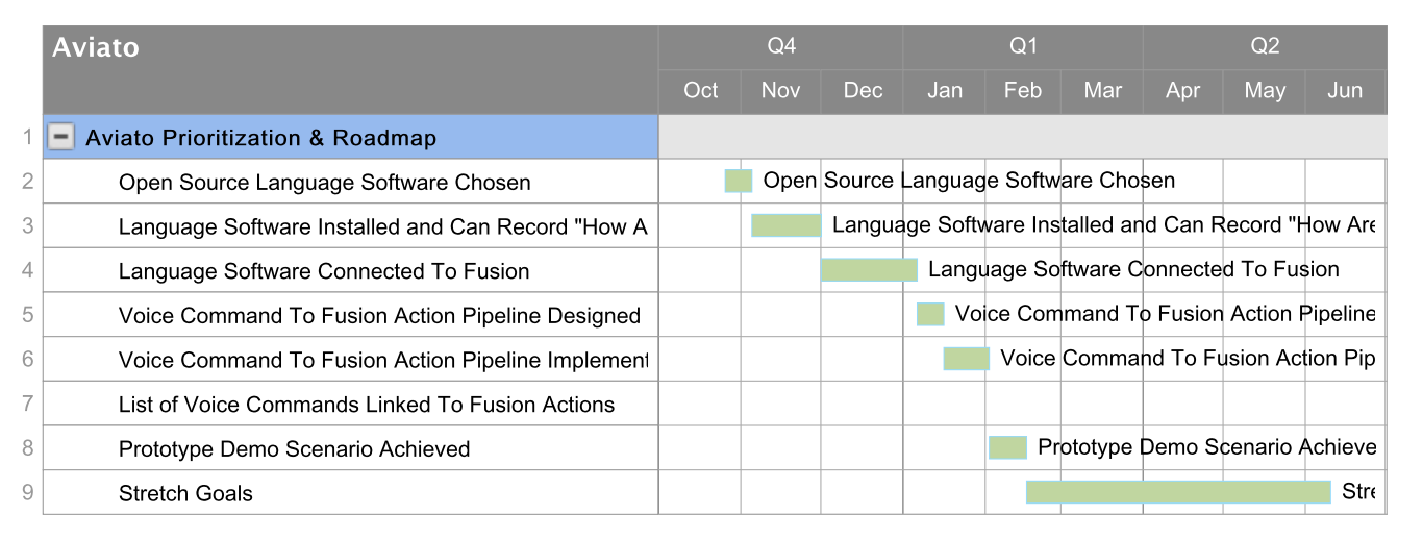
\includegraphics[width=1\textwidth]{ganttChart.eps}
			%Changed Gantt chart to be modifiable.
			\begin{ganttchart}[
				y unit title=0.4cm,
				y unit chart=0.5cm,
				vgrid,
				hgrid,
				title left shift=.05, 
				title right shift=.05, 
				title height=1, 
				group right shift=0
				]{1}{24}
				\gantttitle{Months}{24} \\
				\gantttitle{January}{4} 
				\gantttitle{February}{4} 
				\gantttitle{March}{4} 
				\gantttitle{April}{4} 
				\gantttitle{May}{4} 
				\gantttitle{June}{4} \\

				
				\ganttbar{MongoDB Creation}{1}{2} \\
				\ganttbar{Module Skeletons Creation}{1}{2} \\
				\ganttbar{Speech-To-Intent Working}{2}{3} \\
				\ganttbar{Text-To-Speech Working}{3}{3} \\
				\ganttbar{Fusion API Mapping}{2}{5} \\
				\ganttbar{Pipeline Connected}{4}{9} \\
				\ganttbar{Create Alpha Demo}{9}{11} \\	
				\ganttbar{Performance Testing}{9}{12} \\
				\ganttbar{Train NLP Modules}{13}{20} \\
				\ganttbar{Create Beta Demo}{17}{24} \\
				\ganttbar{Smart Assistant Stretch Goal}{15}{23} \\
				\ganttbar{Engineering Expo}{24}{24}
				
			\end{ganttchart}
			\captionsetup{justification=centering}
			\caption{\botname Development Schedule}
			\label{fig:developmentSchedule1}
		\end{center}
	\end{figure}

			
\section{Conclusion}
	This document has described Kora's development roadmap.
	This document explains the components Kora is broken up in to, and what each are responsible for.
	Above is a Gantt chart which holds a loose development schedule that the Kora developers will abide by.
	There is a change history table at the beginning of this document which will tell the story of any modifications made to the design in this document.



%\bibliographystyle{IEEEtran}
%\bibliography{references.bib}



\end{document}
